\chapter{书籍模板}
\label{chap:main}

最近在阅读两弹一星功勋,为调校模板段落布局,特引入郭永怀先生介绍文字以纪念。

%--
\section{郭永怀先生}

郭永怀(1909年4月4日-1968年12月5日),山东荣成人,中国流体力学家。1999年颁发两弹一星功勋奖章受勋23位科学家之一,主导两弹一星之中原子弹的力学研究。

本科为北京大学物理系转学生,考获庚子赔款出国,最终取得加州理工学院博士学位,师从空气动力学权威西奥多·冯·卡门,读博认识同门师兄钱学森。1946年另一同门师兄William R. Sears在康乃尔大学创航天工程研究生院,郭永怀为创院教员,后升任教授。1956年返国,1958年中国科学技术大学创校时郭永怀担任化学物理系创系系主任。1960年经钱学森力荐,任第二机械工业部第九研究所副所长,主导原子弹的力学研究。1968年坠机亡,死前与护卫紧抱刚获得的氢弹实验数据。

\subsection{简历}

1909年4月4日出生于山东省荣成县。1930年,郭永怀入南开大学预科二年乙组读书,次年8月升入南开大学理科,决心攻读物理学。南开大学当时没有物理系,他打听到电机系有一位物理学教授叫顾静徽,就投到她的门下,成了她唯一的物理专业的学生。顾非常赏识这位好学不倦的学生,为他单独开课。曾在南开大学任教的饶毓泰归国后到北京大学任教,郭永怀仰慕饶毓泰,顾静徽推荐他转学北京大学。1933年,郭永怀通过北京大学入学考试,考入北京大学物理系,1935年毕业。1939年考取中英庚子赔款出国留学名额,1940年赴加拿大多伦多大学应用数学系学习,半年后获硕士学位。1941年到美国加州理工学院师从空气动力学权威西奥多·冯·卡门教授研究可压缩流体力学,1945年获博士学位后留任研究员。1946年起在美国康乃尔大学任副教授、教授。

郭永怀在跨声速流领域和奇异摄动论方面有重要贡献;与钱学森共同发表的论文《可压缩流体二维无旋亚声速和超声速混合型流动及上临界马赫数》提出“上临界马赫数”的概念。郭永怀还发表了《跨声速流的稳定性》、《可压缩流体二维无旋跨声速流动》、《绕翼型的二维跨声速流》、《论二元光滑跨声速流的稳定性1》等跨音速研究论文。郭永怀还发展了奇异摄动法,即PLK方法(庞加莱-莱特希尔-郭永怀方法)。

中国抗日战争胜利后,胡适任北大校长,积极发展北大工科。饶毓泰向胡适推荐正在美国任教的郭永怀、朱兰成、马大猷等青年才俊,同时提议由钱学森担任应用力学系主任。后因钱学森暂时无法离美而未果。新中国成立后,受钱学森之邀返中国,郭永怀夫妇离美前,在赵元任家吃告别晚餐。胡适感叹说:“像郭永怀这样的人都要回国了,真是人心所向啊。”1956年10月回国后任中国科学院力学研究所研究员、副所长。1957年任中国力学学会副理事长,同年聘为中国科学院数学物理学化学部学部委员。他是中国大陆力学事业的奠基人之一,在力学、应用数学和航空事业方面有卓越贡献,是科技工作的领导人和组织实施者。1958年,中国科学技术大学创建了化学物理系,郭永怀担任首任系主任、教授。

1960年5月调任第二机械工业部北京第九研究所(1964年2月改为第九研究院)副所长、副院长。在中国原子弹、氢弹的研制工作中,经钱学森推荐,领导和组织了爆炸力学、高压物态方程、空气动力学、结构力学和武器环境实验科学等研究工作,解决了一系列重大问题。

1968年12月5日,郭永怀从青海省执行任务返回北京时,在飞至北京上空约400米高度时飞机突然因发动机故障而坠毁。郭和同机警卫当场丧生。在清理飞机遗骸时,人们发现郭永怀和他的警卫牟方东紧抱在一起,两人身体之间紧夹着刚刚获得的氢弹试验数据。他们二人的骨灰埋藏于中国科学院力学研究所中郭永怀的塑像下。1999年被授予“两弹一星功勋奖章”,是该群体中唯一一位获得“烈士”称号的科学家。

1982年12月,科学出版社出版了《郭永怀文集》。1985年,郭永怀补授予一项国家科学技术进步奖特等奖。1999年,郭永怀被追授予研制“两弹一星”有突出贡献的科技专家,并荣获两弹一星功勋奖章。2003年9月18日中国科学技术大学创办45周年之际,郭永怀的遗孀李佩将这枚勋章捐赠中国科学技术大学。

%--
\subsection{怀佩道故,大爱无疆:怀念郭永怀和李佩先生}

此文原载于科学网,作者系中科院自然科学史研究所科研人员。

以身许国、大爱无疆。2017年4月5日,郭永怀、李佩合葬仪式在京举行。“云山苍苍、江水泱泱、先生之风、山高水长”,范仲淹的名言成为后人对两位先生永远的怀念。郭永怀和李佩的骨灰将合葬于中科院力学所郭永怀雕像下,这个季节院内正盛开着郭先生生前最喜爱的迎春花。

2017年1月12日,我国“两弹一星”元勋、中国科学院学部委员郭永怀先生的夫人、九十九岁高寿的李佩先生仙逝。郭永怀和李佩先生热爱祖国,服务人民,追求真理,代表着中国真正的知识分子,他们永远活在我们心中。今年清明(4月4日)恰逢郭永怀先生一百零八岁诞辰,谨以此文怀念我们敬爱的郭永怀先生和李佩先生这对科学界伉俪。

1946年,郭永怀在加州理工学院跟从冯·卡门获得博士学位,应师兄西尔斯(W.R. Sears)之邀,到康奈尔大学工作,成为该校航空研究生院的奠基人之一。一年之后,端庄贤淑、风华正茂的李佩来到康奈尔大学工业与劳工关系学院学习。在一次郭永怀关于航天的学术报告会上,二人得以相识。他们有着北京大学和西南联大的共同过往,又都颇好古典音乐,很自然地收获了爱情。1948年,二人喜结连理,李佩治家,郭永怀埋头科研,创造出“ PLK 方法”等传世之作。1951年8月,爱女郭芹降生,一家三口平静而快乐。

1956年9月,在钱学森召唤下,早已归国心切的郭永怀和李佩一家回到祖国,郭永怀被任命为中科院力学所副所长,一家人被安排住进位于中关村的中科院特级专家楼,与钱学森家和钱三强家相邻。少言的郭永怀本来酷爱集邮和音乐,工作的繁忙使他再无暇顾及,而是豪情满怀地投入科研工作。1957年6月7日,郭永怀在《光明日报》发表署名文章,说“我作为一个中国人,有责任回到祖国,和人民一道,共同建设我们美丽的山河”,鼓励还留在美国的同学和朋友们快快回国。

他每天很早赶到所里,晚上、周末都经常可以见到他在办公室忙碌的身影。1958年,在钱学森调往国防部门和钱伟长被打成“右派”后,郭永怀实际领导着力学所。他牢牢把握依工程科学建所的基本方针,在混乱的年代里,尽力保护力学所一批科研方向得以维持。经钱学森的极力推荐,他介入“两弹一星“研制,担任国防部九院副院长,频频往返于青海和北京之间。由于高原反应,他的身体多有不适,还不到50岁头发已经花白,但仍坚持奋战在第一线。

李佩先是担任了中科院行政管理局西郊办公室副主任,建设起了西点屋、医务室、小学和食堂,后于1961年2月,被调到中国科学技术大学外语教研室教英文。她心知他正在从事保密的研究工作,从不过问内情,只是在工作岗位上默默耕耘,照顾家庭,毫无怨言。郭永怀包里总有个苹果,那是李佩给他预备的点心。郭永怀重家庭情义,她便每月按时邮寄80元生活费给他荣成渔村的兄嫂。工作再忙,这对夫妇都事无巨细地关心着研究生和助手的学习和生活,常邀请他们来家中做客。1965年,郭永怀和李佩将家中存款和公债4万8千余元捐赠给力学所。

时隔多年后,郭永怀以烈士身份被授予“两弹一星”功勋奖章,李佩才获悉原来丈夫曾从事国防尖端武器研制,是“两弹一星“元勋中唯一一个在原子弹、导弹和卫星三个领域均有重要贡献的科学家。

“文革“后,郭永怀因参与国防研究,被中央指定保护起来,家人却没有同等待遇。1968年,李佩因在重庆白区工作和美国留学的经历,被作为美国特务在中国科学技术大学的牛棚里开始遭受了长期的“隔离审查”。9月,被父母视为掌上明珠的郭芹“初中还没毕业便上山下乡“,到内蒙古农区做了一名知青。10月3日,郭永怀离开北京赴青海核试验基地,从此一家人分处三地。

在凄风苦雨的年代,人与人相处战战兢兢如履薄冰,郭永怀和李佩却以最善良的心牵挂着别人。“文革”初期,力学所林鸿荪、杨友(原名杨友鸾)夫妇也同样受到了冲击,郭永怀和李佩大胆接纳他们搬到家里合住。1968年12月5日,郭永怀因发现了重要的实验数据,也担心着李佩的安危,与警卫员一同乘坐小飞机赶赴北京。李佩迟迟未见人归,却等来了丈夫遭遇空难的噩耗。相伴廿载的爱人壮年西去,她将所有苦痛和眷恋深埋心底,人前从未流泪。此后,郭芹回到内蒙古插队,因健康受到损害而于1970年病退回京,以烈士子女身份进入中科院力学所工作。其时李佩已随中国科学技术大学迁至合肥,继续受审。直到1973,李佩才被允许春节时回北京探亲。林鸿荪听说郭永怀去世后自杀,精神受到刺激的杨友得到了李佩的悉心照料。

1976年,李佩终获自由回到北京,用行动谱写了灿烂的后半生。她起初给中科院力学所等机构教授英语培训班,1978年,中国科学技术大学研究生院首任院长严济慈委任她负责英语教学的领导工作。她教学极度认真负责,自编教材,制定教学和考试大纲。1979年中美正式建交后不久,李佩便向学生介绍美国大学招收研究生办法,鼓励大家自费留学。为配合李政道教授发起的中美联系招考物理研究生(简称CUSPEA)项目,自1980年起,她负责了9年的 CUSPEA 英语测试。她在英语教学中开创了“应用语言学”。她如一位慈祥的母亲,关爱着国内外学子的成长,希望将他们培养成引领科技前沿的精英,桃李满天下。在她的努力下,中科院于1986年9月正式成立了科技翻译工作者协会,促进了中外科技交流与科学传播事业的发展。

1980年,郭芹移居美国,家中只剩李佩一人。1986年春,李佩从中科院研究生院教学岗退而不休,一直到80岁还在站着给博士生上英语课。本以为生活可以一直平静地过下去。时针指到1994年,郭芹在美国突患癌症,也许一个初中生在美国的生活并不如意,也许早年上山下乡造成的身体损害有了后果,两年后郭芹在北京病故。公私分明的李佩并未将女儿骨灰与父亲合葬,而是将骨灰撒入昆明湖。在中年丧夫的打击后,我们怎能想象她又可以承受老年丧子的大不幸呢?可第二天她就提着录音机去给研究生上课,只是看起来更加清瘦,声音略微嘶哑。

她全身心投入到火热的社会工作中去,从玉泉路到中关村,从中科院南区到北区,她瘦小的身影一直奔波,成为一盏“中关村的明灯”。为了帮老一辈科技工作者安度晚年,她于1995年组织成立了“中关村老年互助服务中心”,当时她最大的心愿是能建成一所中科院老年公寓。1996年至2010年,在她强大的人格魅力的感召下,每周五的中关村讲座邀请来一大批知名专家学者,讲座包容并蓄,文理齐飞,精神矍铄、气质优雅的她亲自主持。没有活动经费,她就自掏腰包给每位主讲人送上鲜花。她每周三在力学所主持的“钱学森科学与教育思想研讨会”,成为远近闻名的思想交流中心。她积极组织的电脑、英语、花艺等各种学习班,也为大家津津乐道。

几十年来,李佩很少提起郭永怀,可她的思念之情比海深,希望郭永怀的科研态度和科学思想能够传承下去。2003年,在中国科学技术大学建校45周年之际,李佩赴安徽,将郭永怀的“两弹一星功勋奖章”赠送给他曾担任过系主任的中国科学技术大学。2007年,这位生活清苦的老人将60万积蓄分赠给中科院力学所和中国科学技术大学的“郭永怀奖学金”。中科院力学所在院内树立一尊郭永怀的汉白玉雕像,李佩将丈夫的骨灰从八宝山烈士公墓迁出,埋葬在雕像下。她没有忘了当年那位与郭永怀一同牺牲的解放军小战士牟方东,将其部分骨灰一同迁葬。她说,郭先生从未离去,就在力学所,在家里,在她身边。

如今,李佩先生这枚“中科院最美的玫瑰”已驾鹤西去,一家人在天堂重逢。“有的人活着,他已经死了;有的人死了,他还活着。”能将自己的生命寄托在他人记忆中,生命仿佛就在加长。4月5日,他们的骨灰将合葬于中科院力学所郭永怀雕像下,这个季节院内正盛开着郭先生生前最喜爱的迎春花。

%--
\section{字体段落}
\label{sec:font}

书籍模板采用方正字体,宋体即正文字体,无需切换。

宋体\verb|\song|:%
郭永怀,山东荣成人,中国流体力学家。
1999年颁发两弹一星功勋奖章受勋23位科学家之一,主导两弹一星之中原子弹的力学研究。

{\hei 黑体\verb|\hei|:%
郭永怀,山东荣成人,中国流体力学家。
1999年颁发两弹一星功勋奖章受勋23位科学家之一,主导两弹一星之中原子弹的力学研究。}

{\kai 楷体\verb|\kai|或仿宋\verb|\fs|:%
郭永怀,山东荣成人,中国流体力学家。
1999年颁发两弹一星功勋奖章受勋23位科学家之一,主导两弹一星之中原子弹的力学研究。}

\begin{itemize}
%\item[初号] {\song\chuhao 郭永怀两弹一星}
%\item[小初] {\song\xiaochu 郭永怀两弹一星}
\item[一号] {\song\yihao 郭永怀两弹一星}
\item[小一] {\song\xiaoyi 郭永怀两弹一星}
\item[二号] {\song\erhao 郭永怀两弹一星}
\item[小二] {\song\xiaoer 郭永怀两弹一星}
\item[三号] {\song\sanhao 郭永怀两弹一星}
\item[小三] {\song\xiaosan 郭永怀两弹一星}
\item[四号] {\song\sihao 郭永怀两弹一星}
\item[小四] {\song\xiaosi 郭永怀两弹一星}
\item[五号] {\song\wuhao 郭永怀两弹一星}
\item[小五] {\song\xiaowu 郭永怀两弹一星}
\end{itemize}

%--
\section{表格明细}
\label{sec:figure}
表格是论文的重要组成部分,详细的表格编制内容繁多,可以参考网上的教程,这里不多赘述。

模板中关于表格的宏包有三个: \textsf{booktabs}、\textsf{array} 和
\textsf{longtabular}。三线表建议使用\textsf{booktabs},
包含toprule、midrule 和 bottomrule三条命令,简单干脆!
它们与\textsf{longtable} 能很好的配合使用。下面来看一个表格实例:
\begin{table}[htb]
  \centering
  \begin{minipage}[t]{0.8\linewidth} % 如果想在表格中使用脚注,minipage是个不错的办法
  \caption[模板文件]{模板文件。如果表格的标题很长,那么在表格索引中就会很不美
    观,所以要像 chapter 那样在前面用中括号写一个简短的标题。这个标题会出现在索
    引中。}
  \label{tab:template-files}
    \begin{tabular*}{\linewidth}{lp{10cm}}
      \toprule[1.5pt]
      {\hei 文件名} & {\hei 描述} \\
      \midrule[1pt]
      bstutf8.bst      & 参考文献 Bibtex 样式文件\\
      bookzh32k.sty    & 书籍模板文件\footnote{表格中的备注} \\
      main.tex         & 主文件\footnote{表格备注} \\
      \bottomrule[1.5pt]
    \end{tabular*}
  \end{minipage}
\end{table}

表 \ref{tab:template-files} 列举了本模板主要文件及其功能,基本上来说论文
中最可能用到的就是这种表格形式了。
请大家注意三线表中各条线对应的命令。这个例子还展示了如何在表格中正确使用脚注。
如果你不需要在表格中插入脚注,可以将minipage环境去掉。
由于\LaTeX{}本身不支持在表格中使用\verb|\footnote|,所以我们不得不将表格放在
小页中,而且最好将表格的宽度设置为小页的宽度,这样脚注看起来才更美观。

%--
\section{绘图插图}

本模板不再预先装载任何绘图包(如 \textsf{pstricks,pgf} 等),完全由你自己来决定。
个人觉得 \textsf{pgf} 不错,不依赖于 Postscript。GUI绘图工具本人强烈推荐\textsf{Ipe}。

一般图形都是处在浮动环境中。之所以称为浮动是指最终排版效果图形的位置不一定与源文
件中的位置对应,这也是刚使用 \LaTeX{} 同学可能遇到的问题。
如果要强制固定浮动图形的位置,请使用 \textsf{float} 宏包,
它提供了 \texttt{[H]}(意思是图片就给我放在这里\textcolor{red}{H}ere)参数,
但是除非特别需要,不建议使用\texttt{[H]},而是推荐使用\texttt{[htbp]},
给\LaTeX{}更多选择。比如图~\ref{fig:ipe}。
\begin{figure}[htbp] % use float package if you want it here
  \centering
  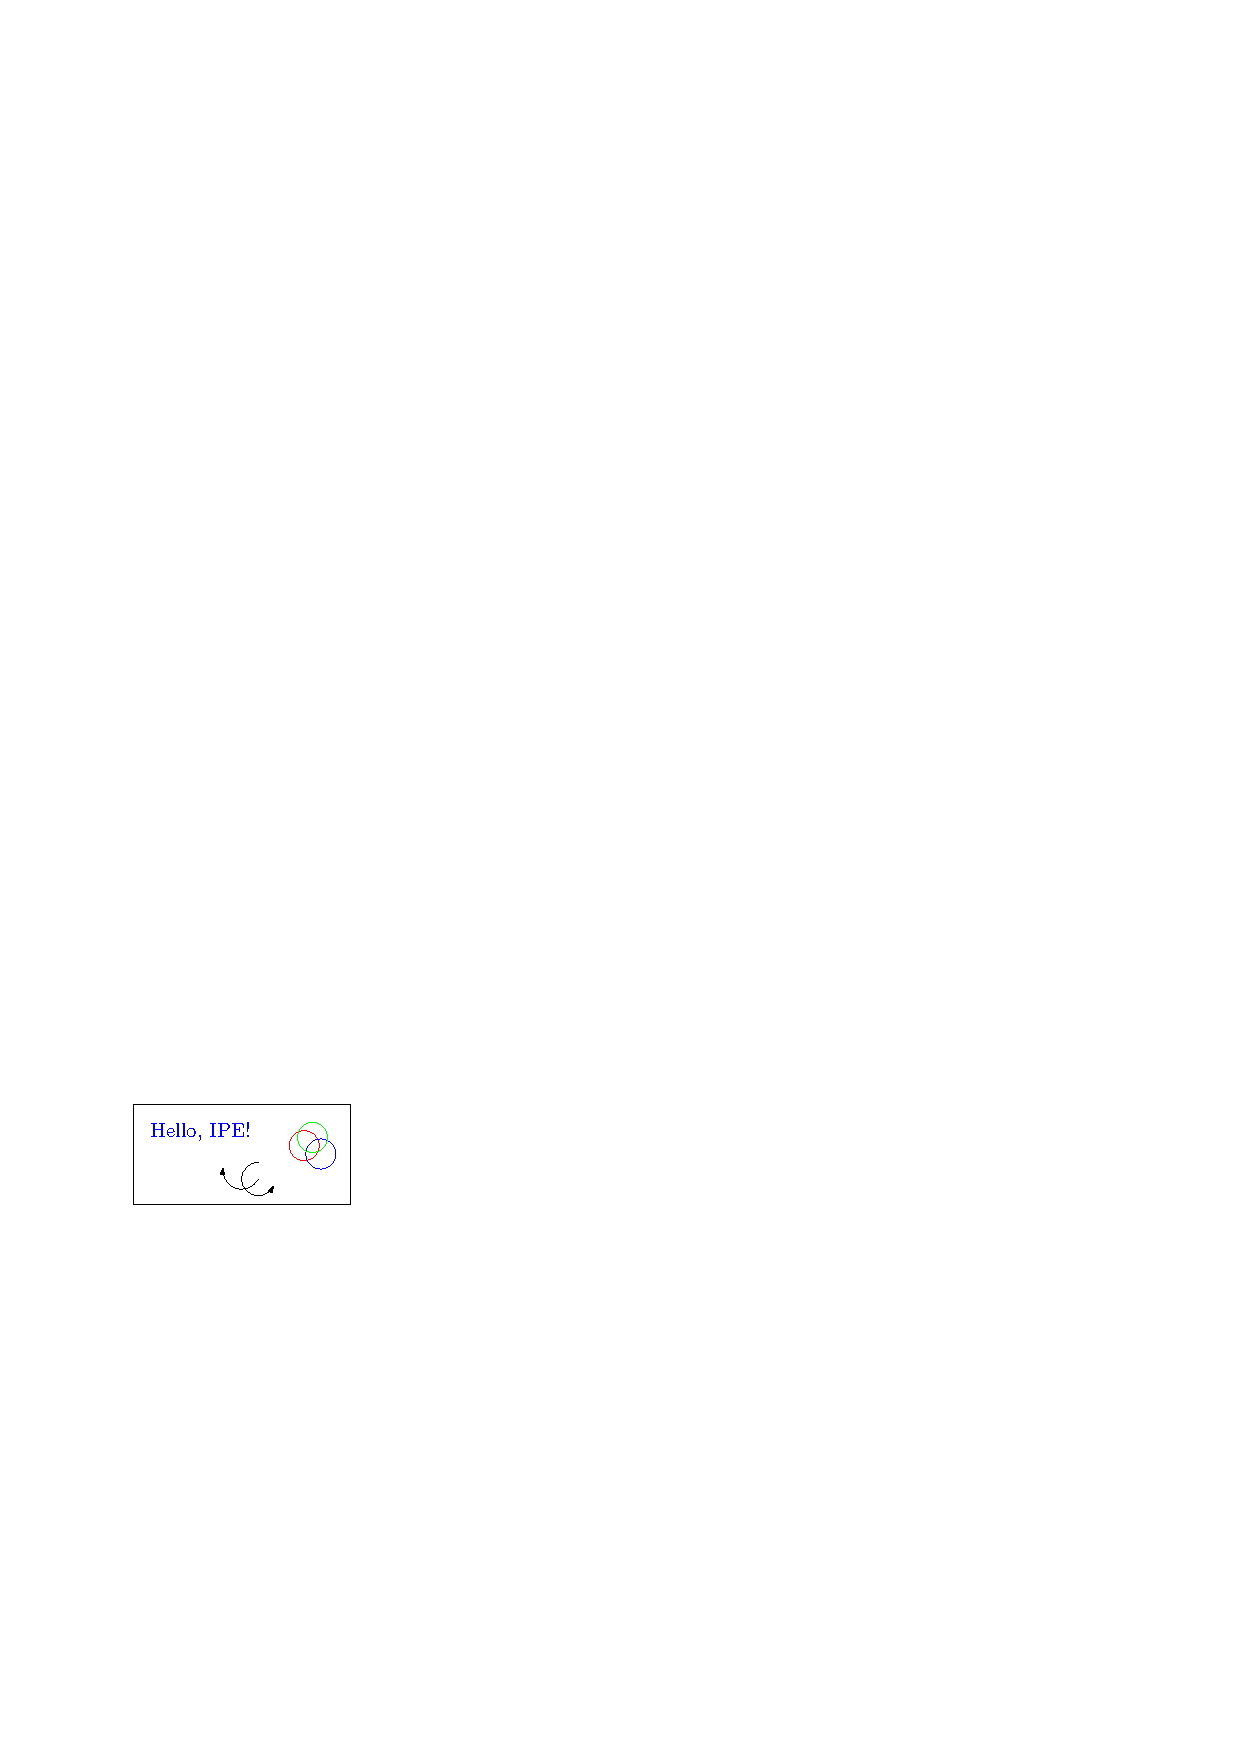
\includegraphics[width=.5\textwidth]{hello}
  \caption{利用IPE制图}
  \label{fig:ipe}
\end{figure}

而下面这个例子显示并排$3\times2$的图片,见图\ref{fig:subfig:3x2}:
\begin{figure}[htb]
\centering
\subfloat[]{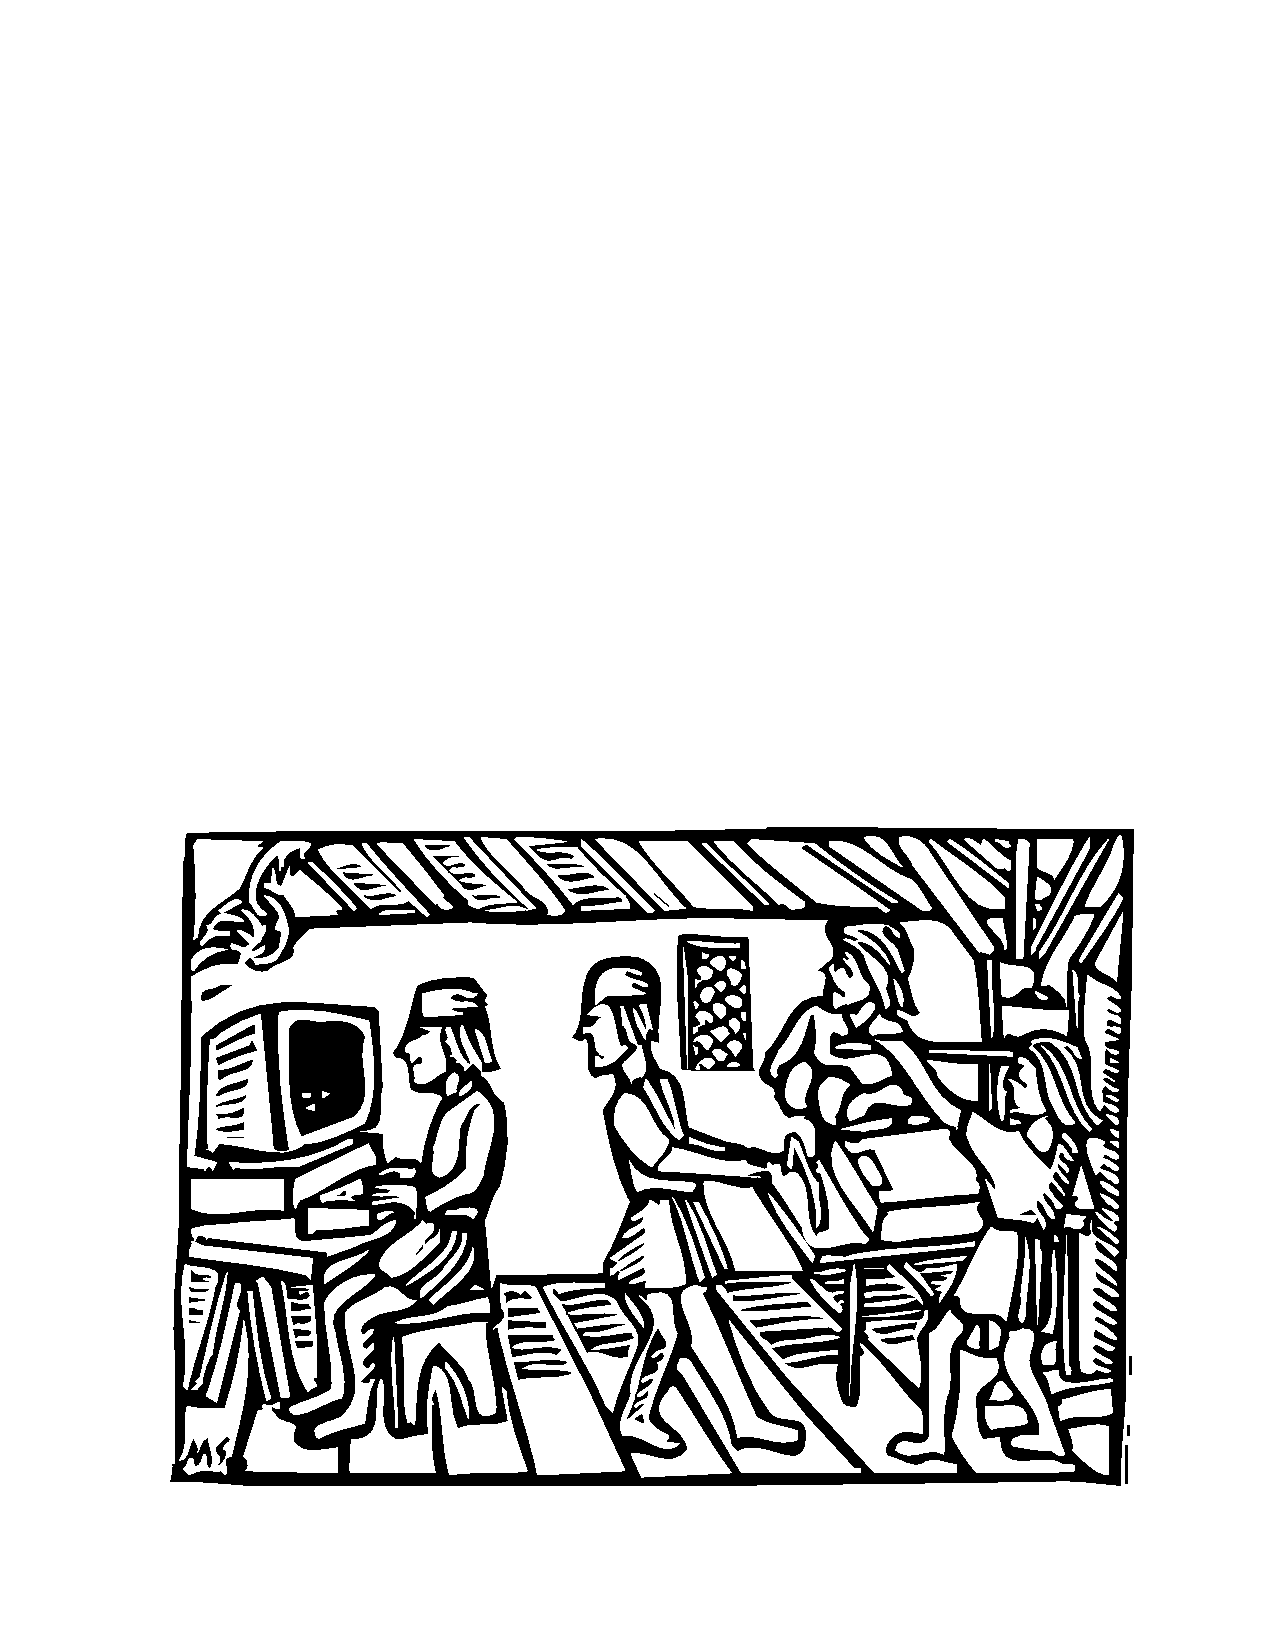
\includegraphics[width=.27\textwidth]{typography}} \qquad
\subfloat[]{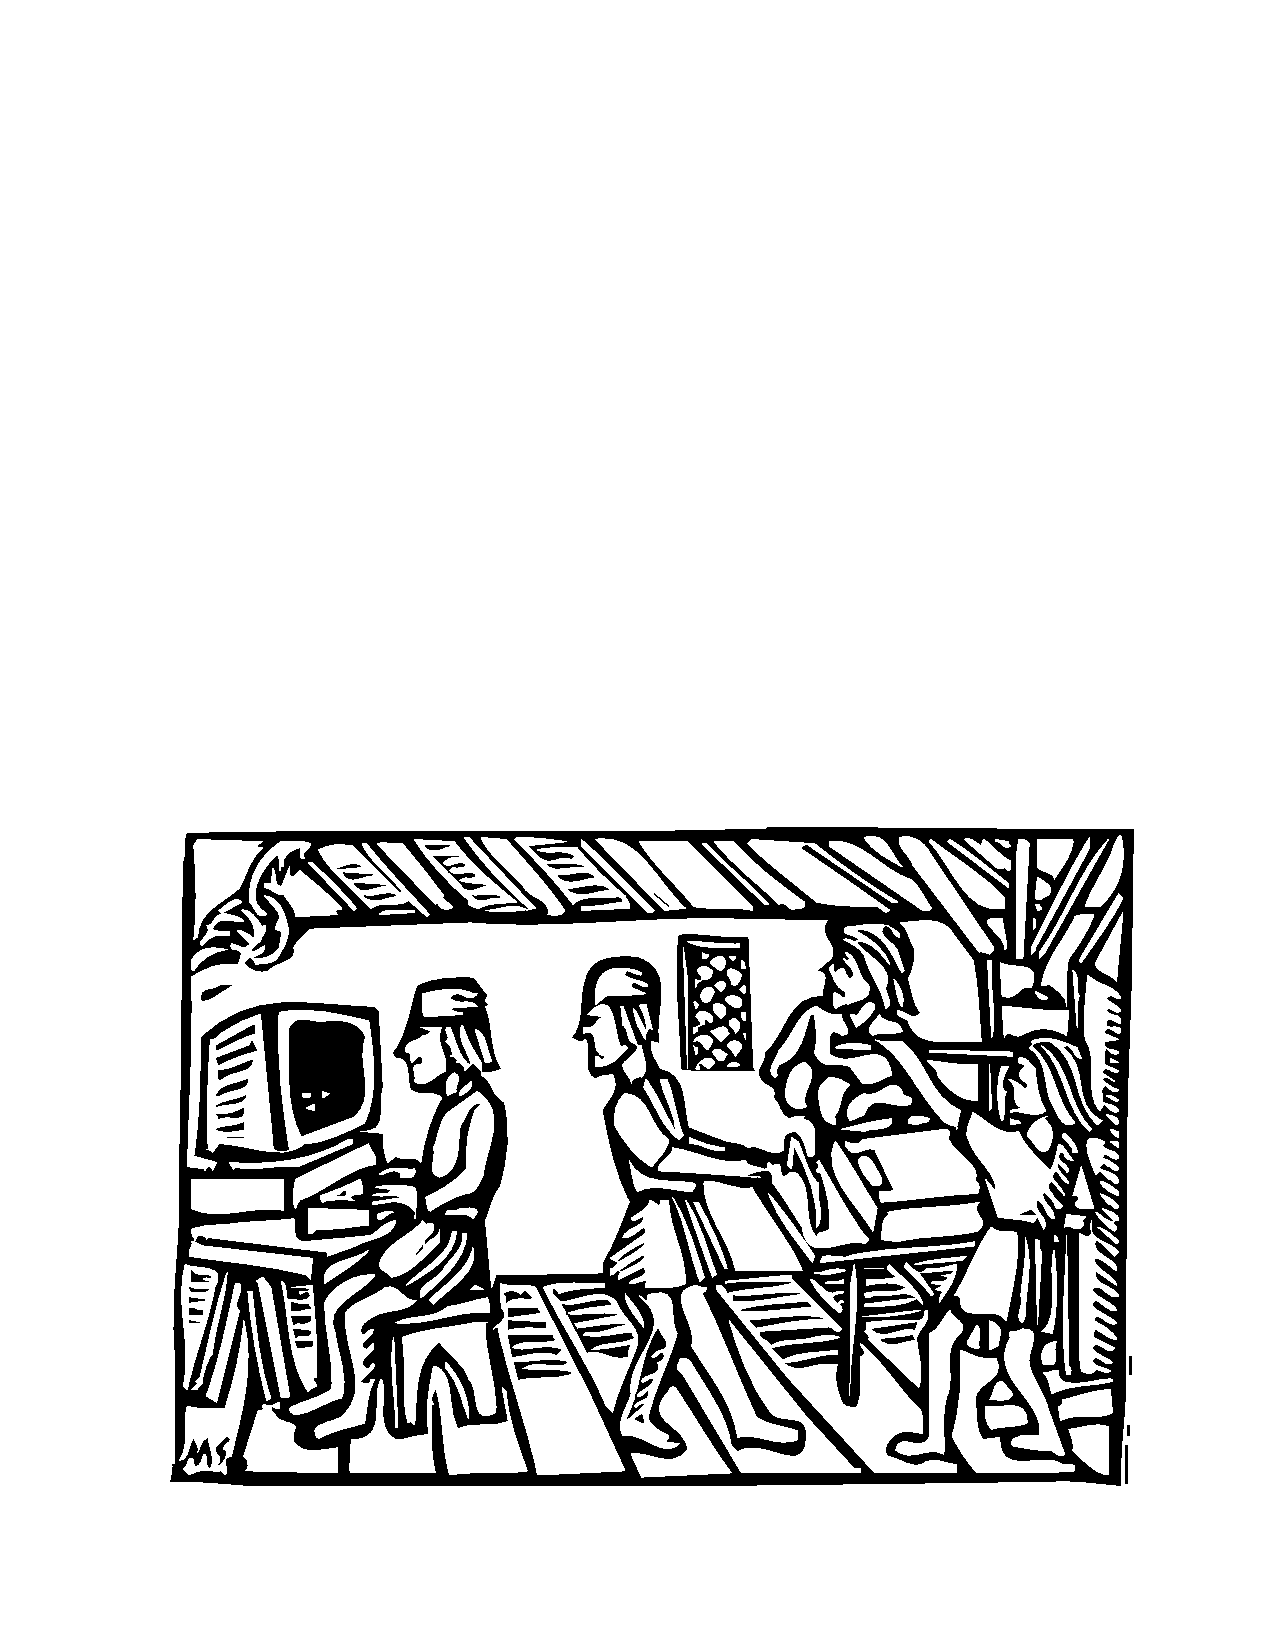
\includegraphics[width=.27\textwidth]{typography}} \qquad
\subfloat[]{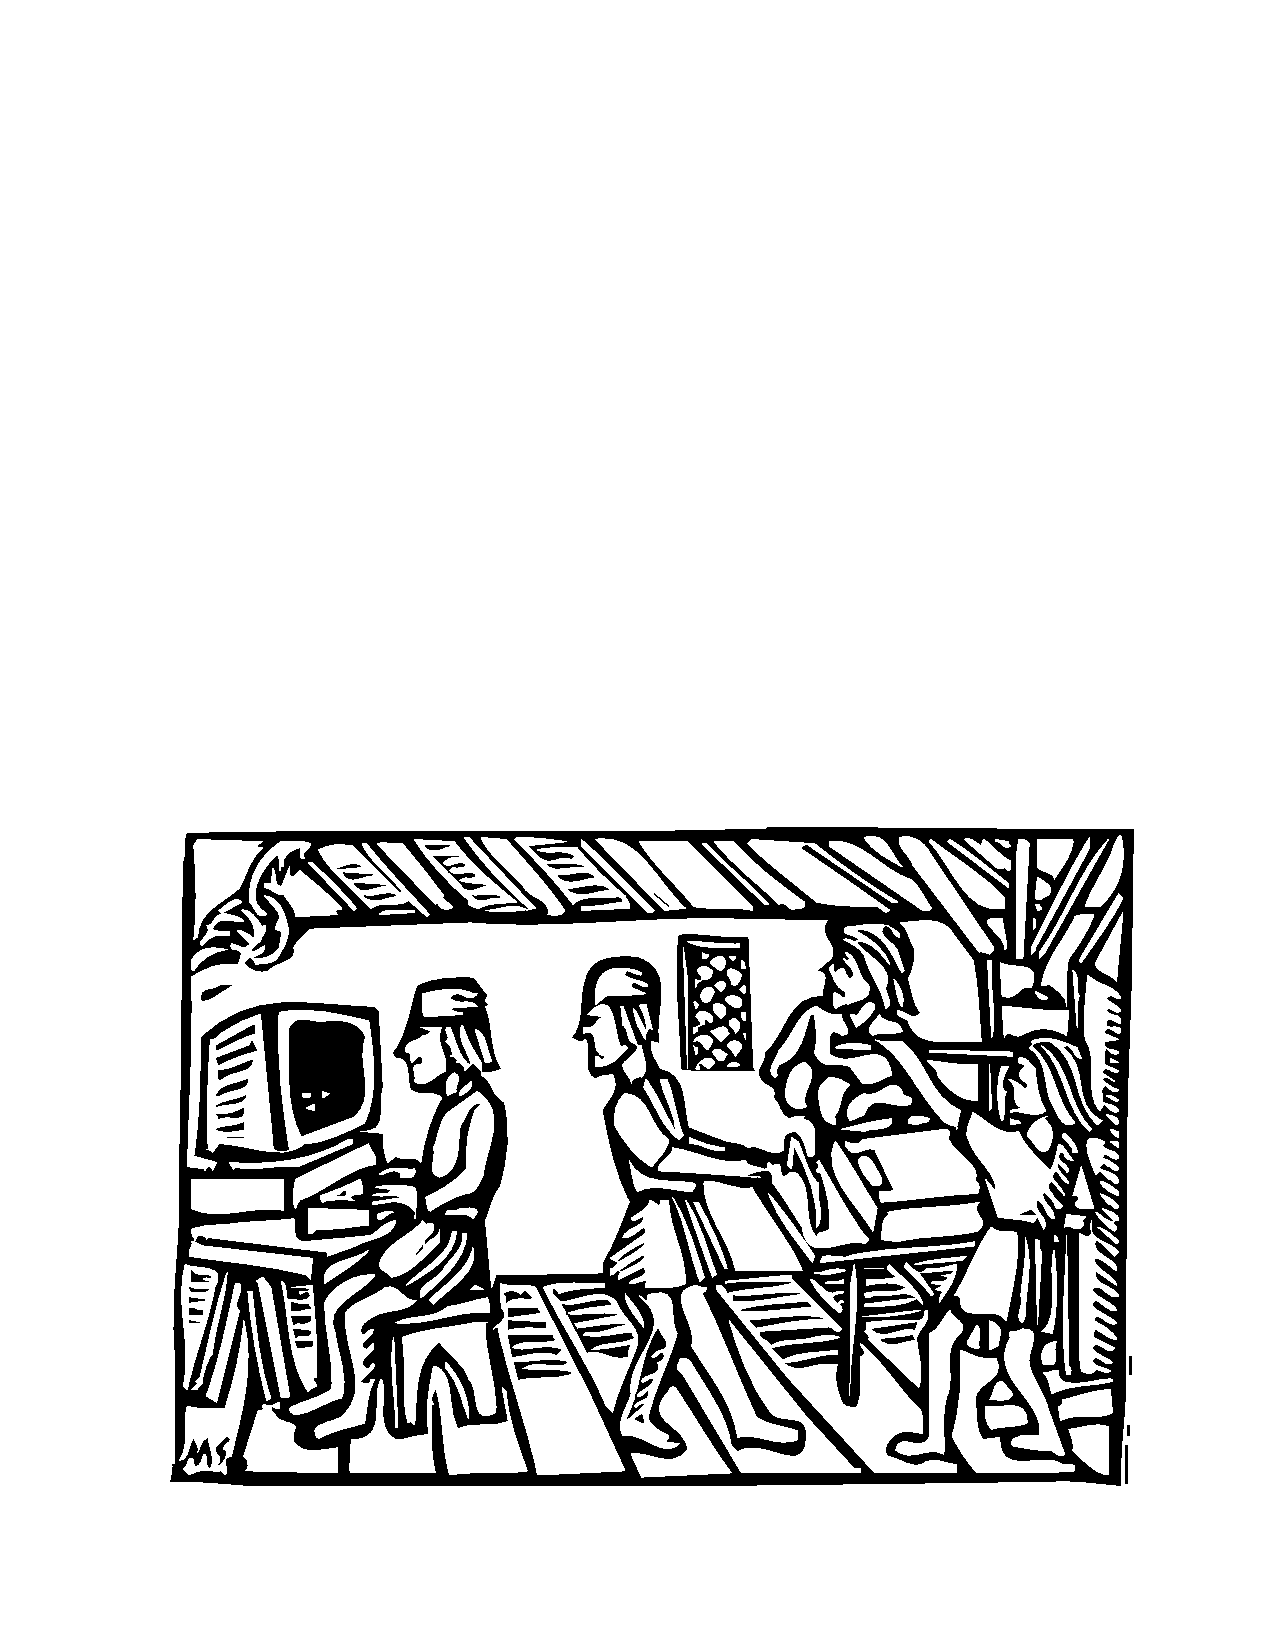
\includegraphics[width=.27\textwidth]{typography}} \qquad
\subfloat[]{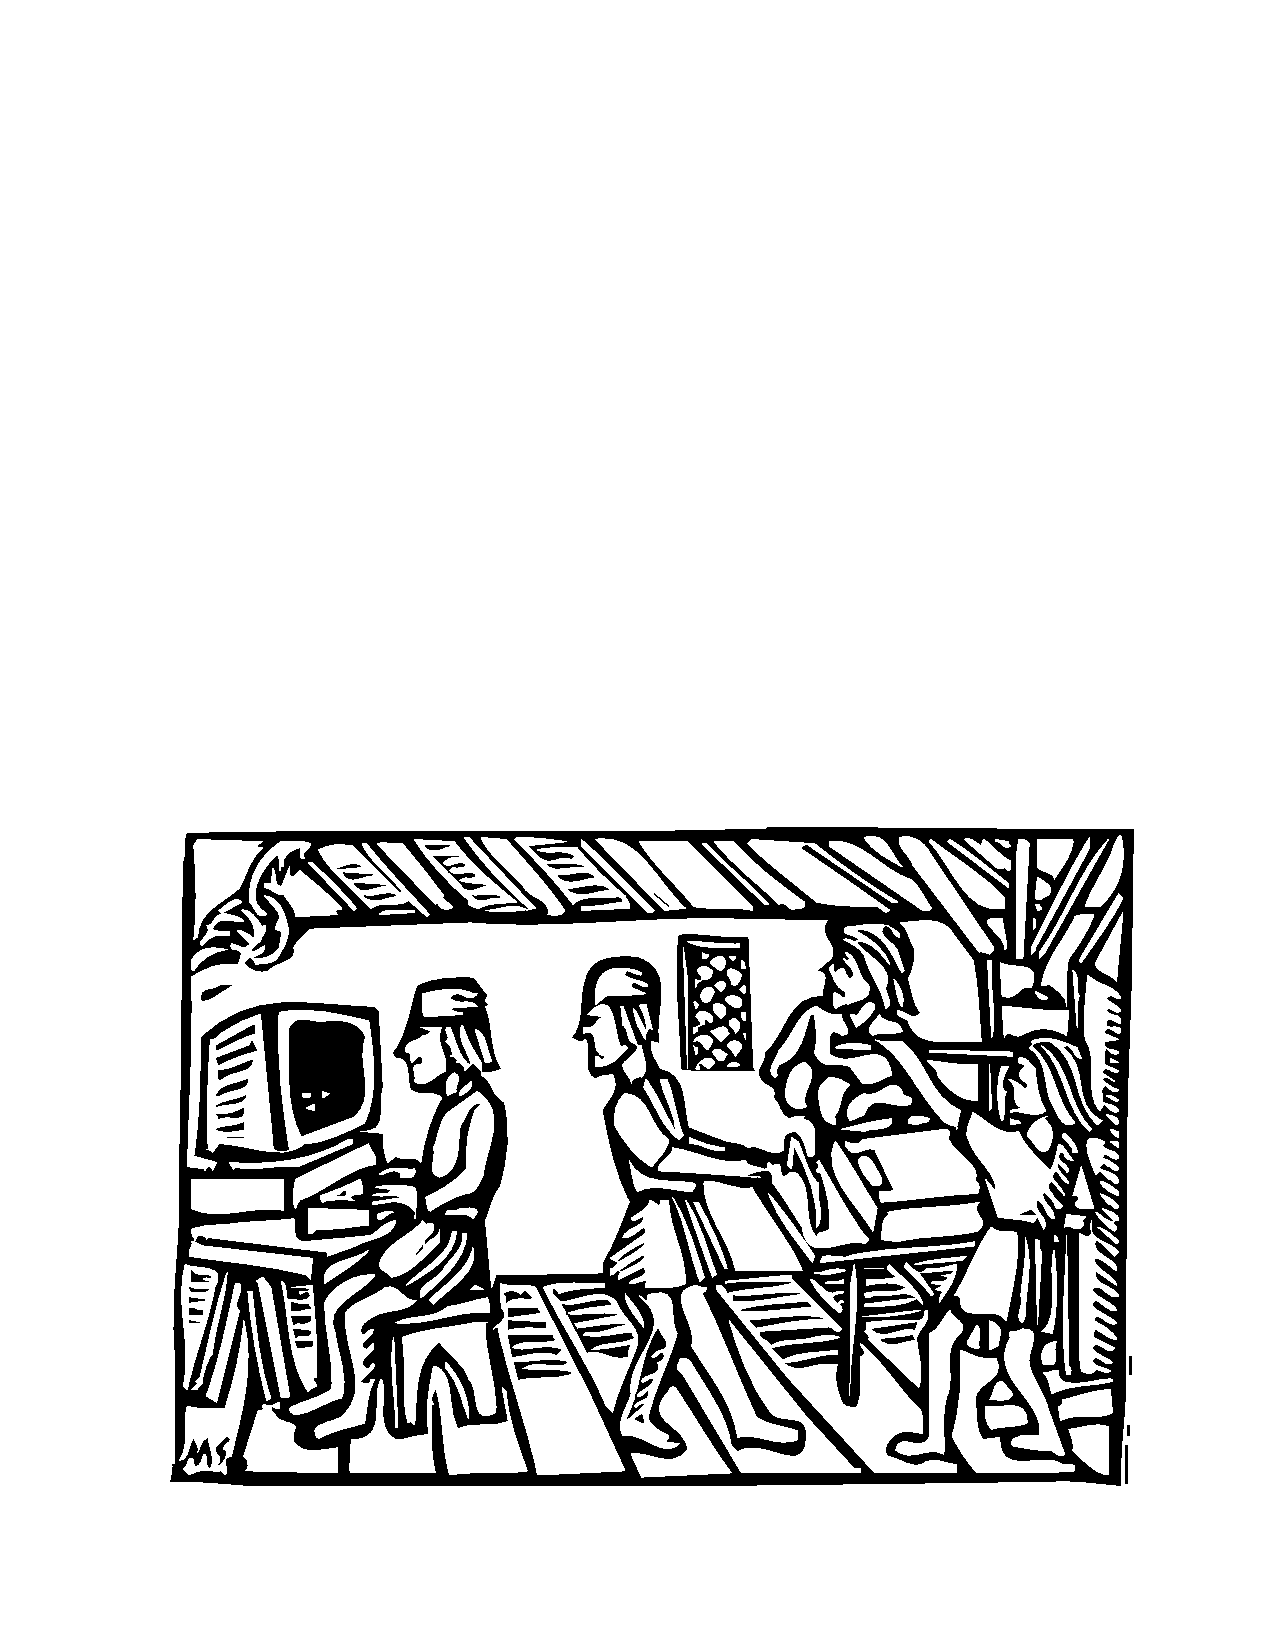
\includegraphics[width=.27\textwidth]{typography}} \qquad
\subfloat[]{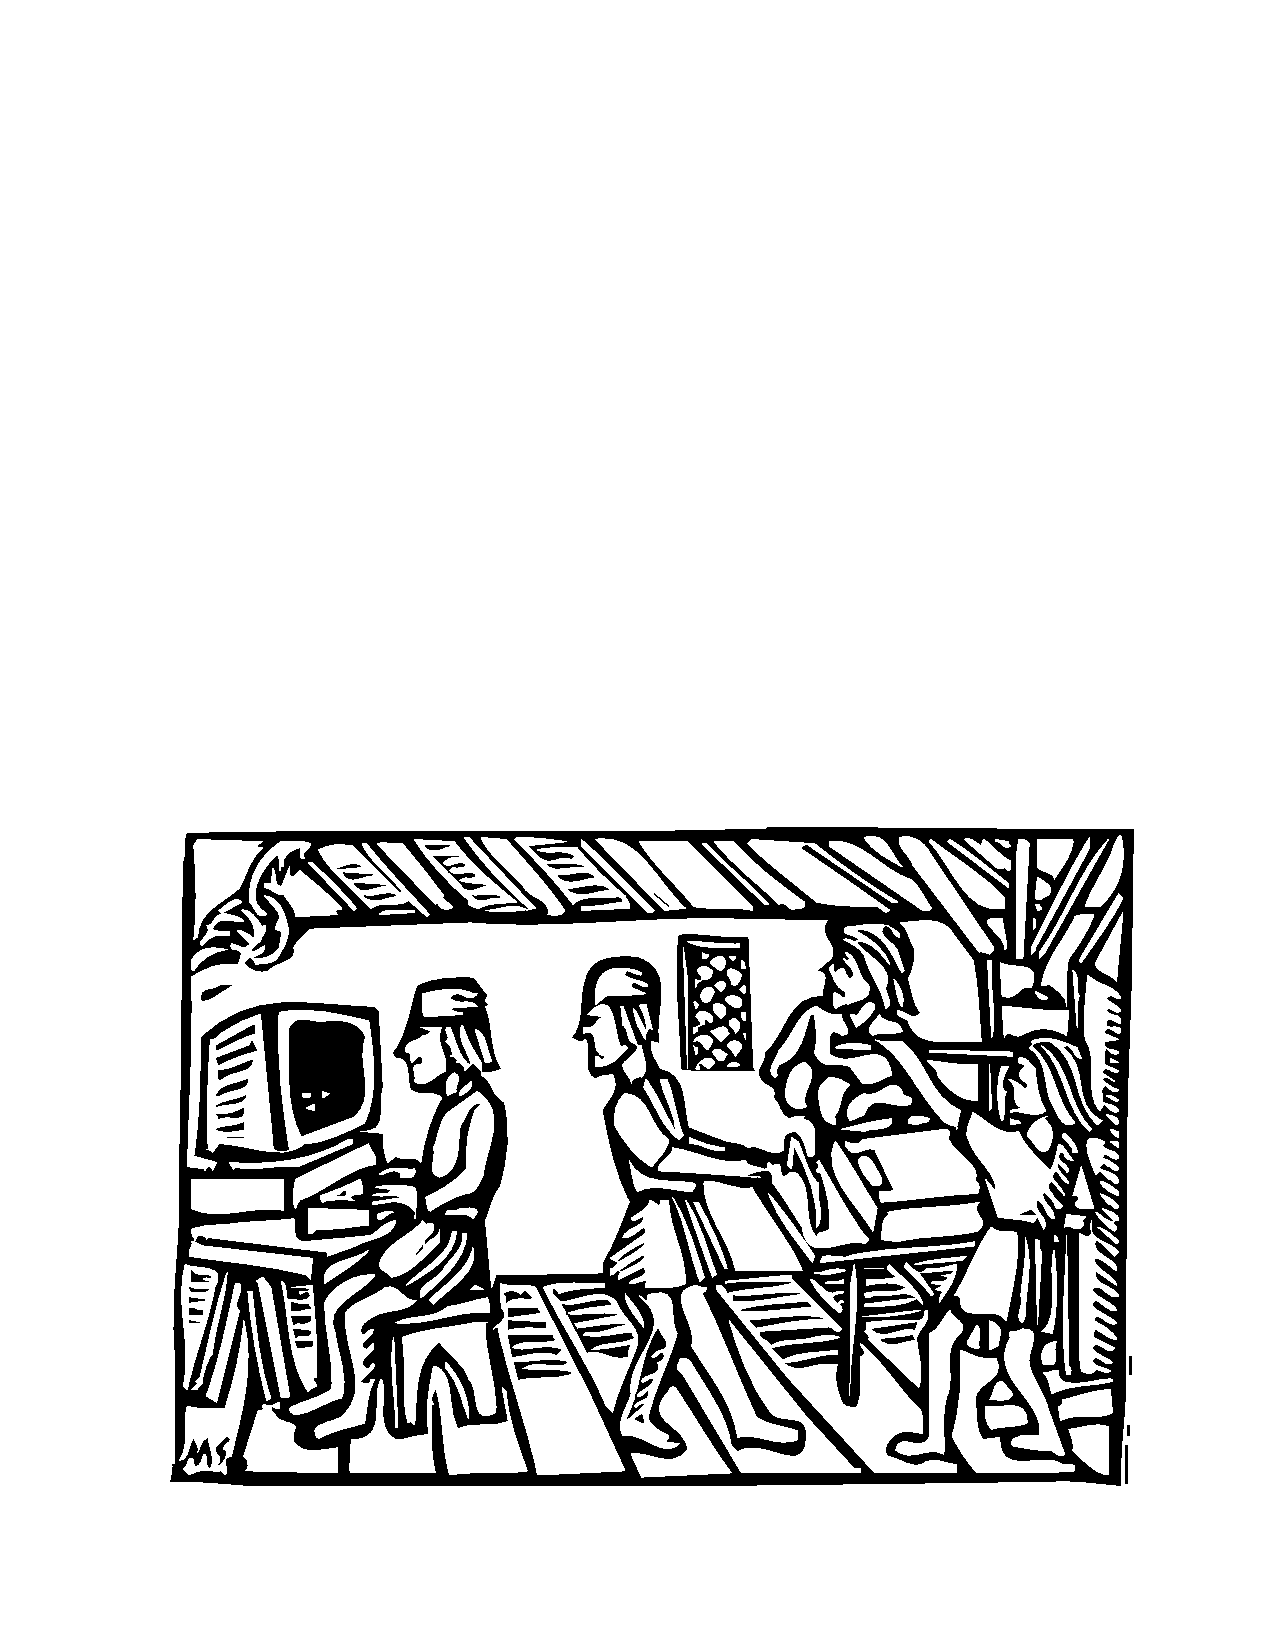
\includegraphics[width=.27\textwidth]{typography}} \qquad
\subfloat[]{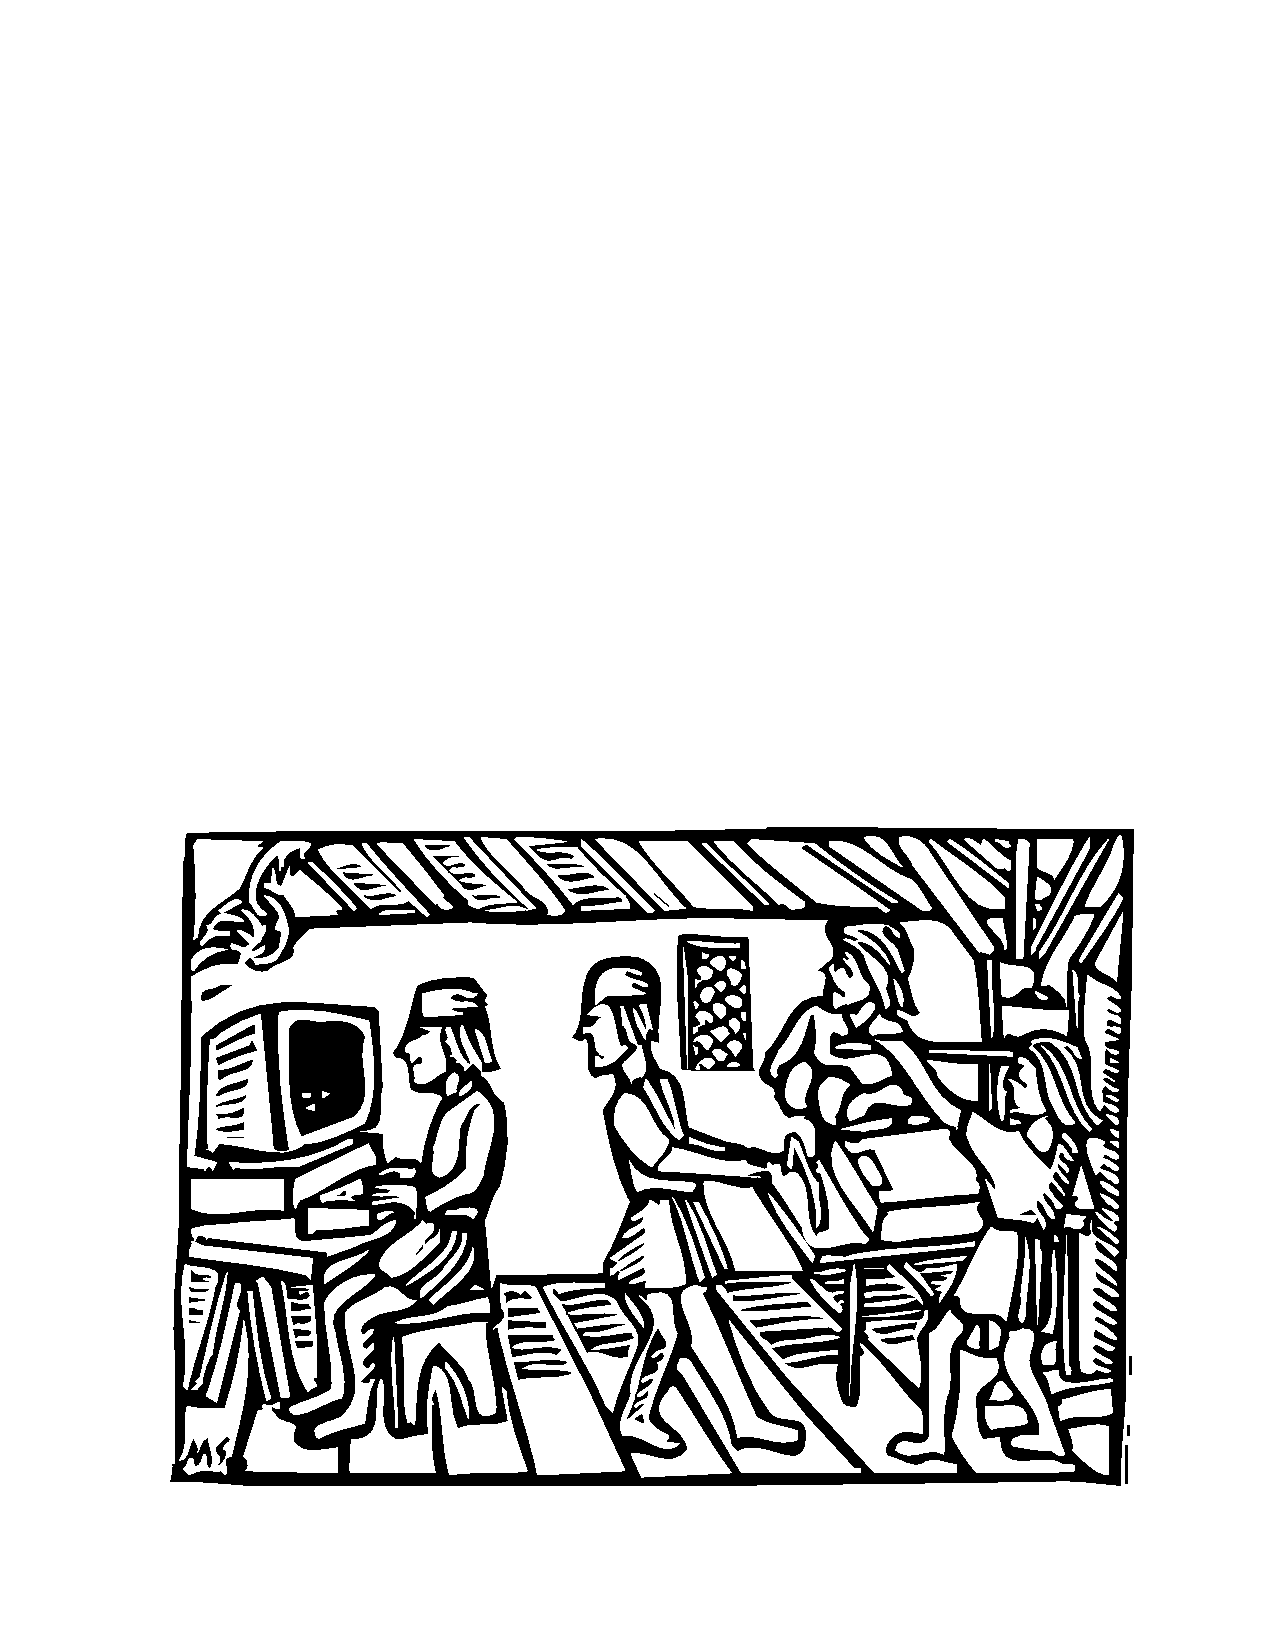
\includegraphics[width=.27\textwidth]{typography}}
\caption{并排图片}
\label{fig:subfig:3x2}
\end{figure}

要注意,图\ref{fig:subfig:3x2}例中
\texttt{qquad}相当于\verb|\hspace{2em}|,也就是2个字符的宽度,约0.08倍页宽,
图片宽度设定为0.27倍页宽是合适的;在该环境中,尽量不要手动换行,所以,不妨自己计算一下!

如果要把编号的两个图形并排,那么小页(minipage)就非常有用了,可以分别参考
图\ref{fig:parallel1}和图\ref{fig:parallel2}。其实这个例子和表格一节中并排
放置的表格一摸一样。
\begin{figure}[htb]
\begin{minipage}{0.48\textwidth}
  \centering
  
\includegraphics[width=\textwidth]{xhh}
  \caption{并排第一个图}
  \label{fig:parallel1}
\end{minipage}\hfill
\begin{minipage}{0.48\textwidth}
  \centering
  
\includegraphics[width=\textwidth]{xhh}
  \caption{并排第二个图}
  \label{fig:parallel2}
\end{minipage}
\end{figure}

图形就说这么多,因为大家在写论文是遇到的最大问题不是怎么把图插进去,
而是怎样做出专业的图片来。

%--
\section{公式定理}
\label{sec:equation}

贝叶斯公式如式~(\ref{equ:chap1:bayes}),其中$p(y|\mathbf{x})$为后验;
$p(\mathbf{x})$为先验;分母$p(\mathbf{x})$ 为归一化因子,
\begin{equation}
\label{equ:chap1:bayes}
p(y|\mathbf{x}) = \frac{p(\mathbf{x},y)}{p(\mathbf{x})}=
\frac{p(\mathbf{x}|y)p(y)}{p(\mathbf{x})} 
\end{equation}

论文里面公式越多,\TeX{} 就越 happy。
\newcommand{\envert}[1]{\left\lvert#1\right\rvert} 
\begin{equation}\label{detK2}
\det\mathbf{K}(t=1,t_1,\dots,t_n)=\sum_{I\in\mathbf{n}}(-1)^{\envert{I}}
\prod_{i\in I}t_i\prod_{j\in I}(D_j+\lambda_jt_j)
\end{equation} 

数学中必不可少的是定理和证明:
\begin{theorem}
  \label{chapTSthm:rayleigh solution}
  假定 $X$ 的二阶矩存在:
  \begin{equation}
         O_R(\mathbf{x},F)=\sqrt{\frac{\mathbf{u}_1^T\mathbf{A}\mathbf{u}_1} {\mathbf{u}_1^T\mathbf{B}\mathbf{u}_1}}=\sqrt{\lambda_1},
  \end{equation}
  其中 $\mathbf{A}$ 等于 $(\mathbf{x}-EX)(\mathbf{x}-EX)^T$,$\mathbf{B}$ 表示协方差阵 $E(X-EX)(X-EX)^T$,$\lambda_1$
$\mathbf{u}_1$是$\lambda_1$对应的特征向量,
\end{theorem}

对于希腊符号使用\verb|mathbf|命令可能有些问题,所以建议对符号
用\verb|bm|加粗,记得用\verb|\up<greek>|切换正体符号,下面看几个例子:
\verb|\gamma|斜体代表变量$\gamma$,\verb|\bm{\upgamma}|正体代表向量$\bm{\upgamma}$,
。\verb|\Gamma|正体代表操作符号$\Gamma$,
\verb|\bm{\Gamma}|正体粗体代表矩阵形式$\bm{\Gamma}$,
\verb|\varGamma|斜体代表变量$\varGamma$。另外对于大小写斜体的加粗可以见$\bm{\gamma}$和$\bm{\varGamma}$,
但是这两种科技论文中很少出现,这里只做测试。
非符号普通向量就用\verb|\mathbf|吧:$\mathbf{x}_k,\mathbf{X}_k$。
完整测试如下$\omega,\bm{\omega},\upomega,\bm{\upomega},\Omega,\bm{\Omega},\varOmega,\bm{\varOmega}$。

\begin{proof}
上述优化问题显然是一个Rayleigh商问题。我们有
  \begin{align}
     O_R(\mathbf{x},F)=\sqrt{\frac{\mathbf{u}_1^T\mathbf{A}\mathbf{u}_1} {\mathbf{u}_1^T\mathbf{B}\mathbf{u}_1}}=\sqrt{\lambda_1},
 \end{align}
 其中 $\lambda_1$ 下列广义特征值问题的最大特征值:
$$
\mathbf{A}\mathbf{z}=\lambda\mathbf{B}\mathbf{z}, \mathbf{z}\neq 0.
$$
 $\mathbf{u}_1$ 是 $\lambda_1$对应的特征向量。结论成立。
\end{proof}

下面来看看算法环境的定义和使用。
我们知道,故障诊断的最终目的,是将故障定位到部件,而由于信号--部件依赖矩阵的存在,因此,实质性的工作是找出由故障部件发出异常信号,
不妨称为源异常信号,而如前所述,源异常信号与异常信号依赖矩阵$\mathbf{S_a}$的全零列是存在一一对应的关系的。因此,我们只要获得了$\mathbf{S_a}$的全零列的相关信息,
也就获得了源异常信号的信息,从而能进一步找到故障源。
通过以上分析,我们构造算法\ref{alg53},用于实现非回路故障诊断。
\begin{algorithm}[htbp]
  \caption{非回路故障诊断算法}
  \label{alg53}
  \begin{algorithmic}[1]
    \REQUIRE 信号部件依赖矩阵$\mathbf{A}$,信号矩阵$\mathbf{S}$,信号状态向量$\alpha$
    \ENSURE 部件状态向量$\gamma$
    \STATE $\mathbf{P}\leftarrow\left(<\alpha>\right)$
    \STATE $\mathbf{S_{a}}\leftarrow\mathbf{P^T}\mathbf{S}\mathbf{P}$
    \FOR{$i=1$ to $S_a$的阶数$m$}
    \STATE $s_i\leftarrow s_i$的第$i$个行向量
    \ENDFOR
    \STATE $\beta_a\leftarrow\lnot \left(s_1\lor s_2\lor \cdots\lor s_m\right)^T$
    \STATE $\beta\leftarrow\mathbf{P}\beta_a$
    \STATE $\gamma\leftarrow\mathbf{A}\beta$
  \end{algorithmic}
\end{algorithm}

第一类故障回路推理与非回路故障推理是算法基本相同,稍微不同的是$\beta_a$的计算。因为第一类故障回路中的信号全部可能是源异常信号,因此我们不必计算
$\beta_a=\lnot \left(\left[s_1\lor s_2\lor \cdots\lor s_m\right]^T\right)$,而直接取$\beta_a=\underbrace{\left[\begin{array}{cccc}1&1&\cdots&1\end{array}\right]^T}_m$,将$\beta_a$代入
算法\ref{alg53},有
\[\beta=\mathbf{P}\beta_a=\mathbf{P}\underbrace{\left[\begin{array}{cccc}1&1&\cdots&1\end{array}\right]^T}_m=\alpha\]
因此一类故障回路的推理算法变得相当简单,例如算法\ref{alg54}
\begin{algorithm}[htbp]
  \caption{第一类故障回路诊断算法}
  \label{alg54}
  \begin{algorithmic}[1]
    \REQUIRE 信号--部件依赖矩阵$\mathbf{A}$,信号状态向量$\alpha$
    \ENSURE 部件状态向量$\gamma$
    \STATE $\gamma\leftarrow\mathbf{A}\alpha$
  \end{algorithmic}
\end{algorithm}

%--
\section{参考文献}
\label{sec:bib}

\textbf{注意:我最终会使用GB2017规范格式。}

当然参考文献可以直接写 bibitem,虽然费点功夫,但是好控制,各种格式可以自己随意改
写,在nudtpaper里面,建议使用JabRef编辑和管理文献,再结合\verb|bstutf8.bst|,
对中文的支持非常不错,格式也很规范。

本模板推荐使用 BIB\TeX,样式文件为 bstutf8.bst,符合学校的参考文献格式(如专利
等引用未加详细测试)。看看这个例子,关于书的\upcite{tex, companion},
还有这些\upcite{Krasnogor2004e, clzs, zjsw},关于杂志的\upcite{ELIDRISSI94,
MELLINGER96, SHELL02},硕士论文\upcite{zhubajie, metamori2004},博士论文
\upcite{shaheshang, FistSystem01},标准文件\upcite{IEEE-1363},会议论文\upcite{DPMG,kocher99},%
技术报告\upcite{NPB2}。中文参考文献\upcite{cnarticle}\textsf{特别注意},需要在\verb|bibitem|中
增加\verb|language|域并设为\verb|zh|,英文此项可不填,之后由\verb|bstutf8|统一处理
(具体就是决定一些文献在中英文不同环境下的显示格式,如等、etc)。
若使用\verb|JabRef|,则你可按下面步骤来设置:
选择\textsf{Options}$\rightarrow$\textsf{Set Up General Fields},
在\verb|General:|后加入\verb|language|就可以了。

有时候不想要上标,那么可以这样\cite{shaheshang},这个非常重要。

